\documentclass[]{report}

\usepackage[utf8]{inputenc}
\usepackage[spanish]{babel}

\usepackage{graphicx}
\usepackage{listings}
\usepackage{hyperref}

% Title Page
\title{PECL3 - Divide y Vencerás}
\author{Miguel Ángel Guerrero y Jorge Guillamón}


\begin{document}
\maketitle

\begin{abstract}
	Memoria de los ejercicios 3, 4 y 6. El código fuente se puede encontrar en este mismo directorio. Todos los ejercicios vienen con probador.
\end{abstract}
\subsection*{Ejercicios 3 y 6 - Búsqueda Binaria}
Hemos planteado la resolución de estos ejercicios mediante una búsqueda binaria. La solución presentada hace uso de dos funciones:
\begin{figure}[h!]
	\centering
	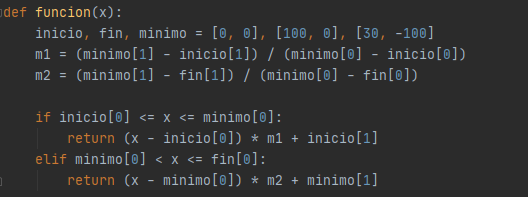
\includegraphics[width=1\linewidth]{1}
	\label{fig:1}
\end{figure}\\
La primera de ellas es una función del tipo que se requiere en ambos problemas: una función definida en un intervalo [a,b], estrictamente decreciente en [a,c] con $a<c<b$ y estrictamente creciente en [c,b].\\
Como se puede apreciar en el código fuente, hemos escogido una función lineal de 2 tramos. 
Cambiando las variables de la primera línea se puede alterar el resultado al gusto.
\\
Finalmente, la función principal del programa, tiene como argumentos: dos enteros, la x inicial y el tamaño del dominio; una función como la de antes, para calcular valores y finalmente el máximo error admisible.
\begin{figure}[h!]
	\centering
	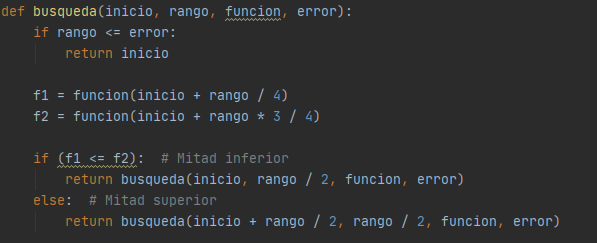
\includegraphics[width=1\linewidth]{2}
	\caption{}
	\label{fig:2}
\end{figure}\\
Como se puede apreciar es una búsqueda binaria al uso. En este caso hemos tomado valores al 1/4 del dominio y 3/4 del dominio para saber a qué mitad dirigirnos en la siguiente iteración. Si $f2 \geq f1$ significa que el mínimo se encuentra en la mitad inferior y viceversa.\newpage

\subsection*{Ejercicio 4 - El robot embotellador}
Para afrontar este problema se ha emparejado el primer tapón con su botella. A continuación, hemos usado esta información para dividir los tapones y botellas restantes en dos grupos según sean mayores o menores que la pareja. Tras esto nos quedamos con 2 grupos que se pueden resolver recursivamente.
\begin{figure}[h!]
	\centering
	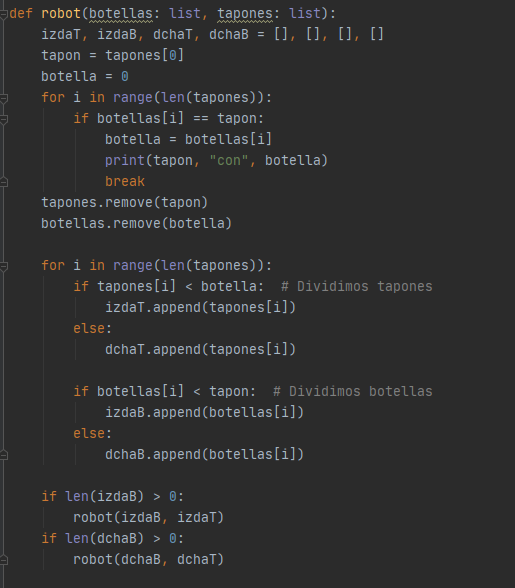
\includegraphics[width=1\linewidth]{3}
	\caption{}
	\label{fig:3}
\end{figure}\\
La salida de la función se hace directamente por pantalla. El programa sacará por pantalla un mensaje cada vez que el robot haya conseguido hacer una pareja.
\newpage
Los probadores generan una lista aleatoria para cada ejecución del programa.
\begin{figure}[h!]
	\centering
	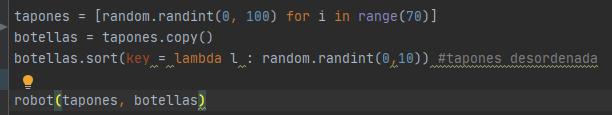
\includegraphics[width=1\linewidth]{4}
	\caption{}
	\label{fig:4}
\end{figure}\\
Las listas se desordenan antes de ejecutarse.

\end{document}          

